\begin{figure}[h!]
\centering
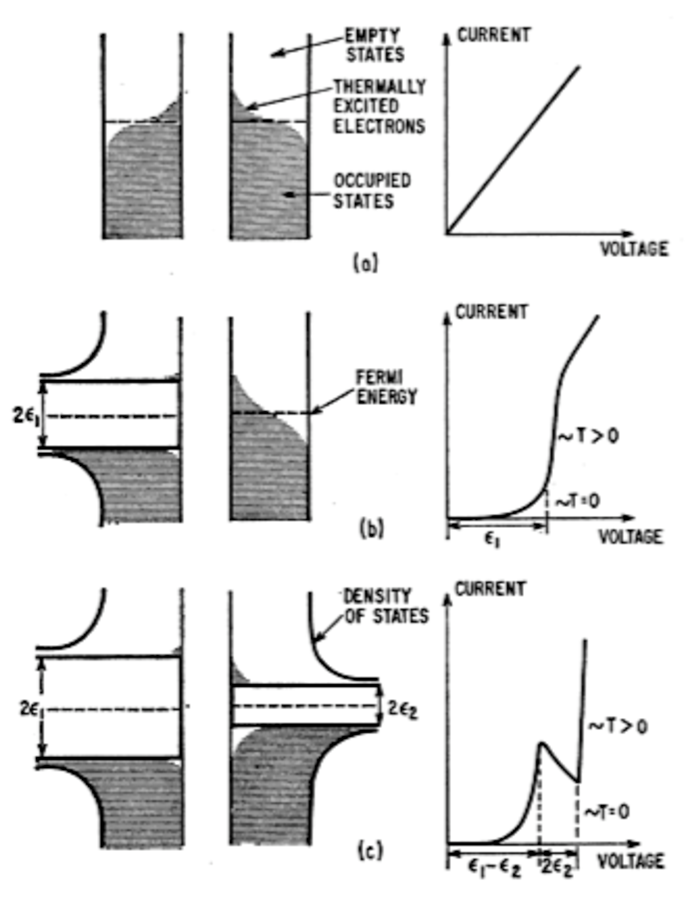
\includegraphics[width=0.45\textwidth]{fermi_levels}
\caption{\small State densities and tunneling currents for three different configurations.
\label{fermi_levels}}
\end{figure}

The transition rate $W$ for an electron from an occupied state in the layer 1 with momentum $\mathbf{p_1}$ to a free state in the layer 2 with momentum $\mathbf{p_2}$ can be calculated by means of the Fermi Golden Rule as follows:
\begin{equation}\label{probability1}
W_{1\to 2}^{1e} = \frac{2\pi}{\hbar} |T_{21}|^2 f(\epsilon_{\mathbf{p_1}}) [1-f(\epsilon_{\mathbf{p_2}})]
		\delta(\epsilon_{\mathbf{p_1}}-\epsilon_{\mathbf{p_2}})\delta_{s_1s_2},
\end{equation}
where $T_{21}$ is the transition amplitude, $ f(\epsilon_{\mathbf{p_1}})$ the probability that the state $\mathbf{p_1}$ is occupied and  $[1-f(\epsilon_{\mathbf{p_2}})]$ the probability that the state $\mathbf{p_2}$ is empty. The conservation of the energy and spin in the transition are also assumed. 

We will assume that the transition hamiltonian does not depend on the spin and couples weakly the electrodes with a small applied voltage (a valid approximation for the voltages used in this experiment). Hence, the total transition rate from the electrode 1 to the electrode 2 will be
\begin{equation}\label{probability3}
W_{1\to 2} = \frac{4\pi}{\hbar} |T|^2 \sum_{\mathbf{p_1},\mathbf{p_2}}  
		f(\epsilon_{\mathbf{p_1}}) [1-f(\epsilon_{\mathbf{p_2}})] 
		\delta(\epsilon_{\mathbf{p_1}}-\epsilon_{\mathbf{p_2}}).
\end{equation}
The transition rate in the opposite way is analogous.

Now we can write explicitly the expression for the current in the $1\to 2$ direction:
\begin{equation}\label{current1}
I = e\ (W_{1\to 2} - W_{2\to 1}),
\end{equation}
that is
\begin{equation}\label{current2}
I = \frac{4\pi e}{\hbar} |T|^2 \sum_{\mathbf{p_1},\mathbf{p_2}}  
		[f(\epsilon_{\mathbf{p_1}})-f(\epsilon_{\mathbf{p_2}})] 
		\delta(\epsilon_{\mathbf{p_1}}-\epsilon_{\mathbf{p_2}})..
\end{equation}

If we replace the summatories by integrals, considering that the momentums form a quasicontinuum, and assuming a voltage difference $V$ between the electrodes that makes $\mu_2-\mu_1=eV$, we get
\begin{eqnarray}\label{current3}
&I& = \frac{4\pi e}{\hbar}  |T|^2 \times
	\nonumber \\
	&\times& \int_{-\infty}^{\infty} d\epsilon\ N_1(\epsilon-eV)\ N_2(\epsilon) [f(\epsilon-eV)-f(\epsilon)],
	\nonumber \\
\end{eqnarray}
where $N(E)$ is the density of states, needed to perform the change from summatories to the integral.

Now three cases can be distinguished: both electrodes are metals in the normal state, only one of them is in the superconducting state and both are in the superconducting state. The only difference between these situations is the shape of the density of states $N(E)$, so it must be replaced by the adequate expression.

%-----------------------------------------------------------------
\subsection{Normal-Normal junction}
For a sufficiently small voltage $V$, the state densities can be considered nearly constant, and equation \eqref{current3} reads
\begin{equation}\label{inn}
I^{NN} = \frac{4\pi e}{\hbar} |T|^2 N_1(\mu)N_2(\mu) eV,
\end{equation}
where we have used the fact that $$ \int_{-\infty}^{\infty}d\epsilon [f(\epsilon-eV)-f(\epsilon)] \simeq eV. $$

From this equation can be derived easily the normal conductance of the junction
\begin{equation}\label{cnn}
C^{NN} = \frac{1}{R^{NN}} = \frac{dI^{NN}}{dV} = \frac{4\pi e^2}{\hbar} |T|^2 N_1(\mu)N_2(\mu).
\end{equation}


%-----------------------------------------------------------------
\subsection{Normal-Superconductor junction} 
The state density for a superconductor can be derived from considering a continuum spectrum of energy levels, and hence
\begin{equation}
N_N(\epsilon) d\epsilon = N_S(E)dE.
\end{equation}

The relation between $\epsilon$ and $E$ in the range of the BCS Theory of Superconductivity is $E_{\mathbf{p}} = \sqrt{\epsilon_{\mathbf{p}}^2 + \Delta^2}$, with $\Delta$ the gap of the superconductor. So we can get
\begin{eqnarray}\label{ns}
&&N_S(E) = N_N(\epsilon) \left | \frac{d\epsilon}{dE} \right | = 
	\nonumber \\
&& = \left\{ 
\begin{array}{ll} 
N_N(\epsilon)\frac{|E|}{\sqrt{E^2-\Delta^2}},	&	|E| > \Delta 	\\ 
0,								& 	|E| \leq \Delta	\\
\end{array}
\right..
	\nonumber \\
\end{eqnarray}

If we replace this state density in \eqref{current3} we get the $I^{NS}$, but only up to $|T|^2$ order. There are high order effects by means of Cooper pair transmission to the superconducting electrode. Neglecting these issues, the current for small voltages is
\begin{eqnarray}\label{ins_previous}
&I^{NS}& = \frac{4\pi e}{\hbar} |T|^2 N_{1N}(\mu) \times
		\nonumber \\
		&\times& \int_{-\infty}^{\infty} dE\ N_{2S}(E) [f(E-eV)-f(E)] =
		\nonumber \\
		&=& \frac{4\pi e}{\hbar} |T|^2 N_{1N}(\mu) N_{2N}(\mu) \times
		\nonumber \\
		&\times& \int_{-\infty}^{\infty} dE\ \frac{|E|}{\sqrt{E^2-\Delta^2}} [f(E-eV)-f(E)].
		\nonumber \\
\end{eqnarray}

It can be expressed in terms of the $C^{NN}$ as follows:
\begin{equation}\label{ins}
I^{NS} = \frac{C^{NN}}{e} \int_{-\infty}^{\infty} dE\ \frac{|E|}{\sqrt{E^2-\Delta^2}} [f(E-eV)-f(E)].
\end{equation}


\begin{figure}[t!]
\centering
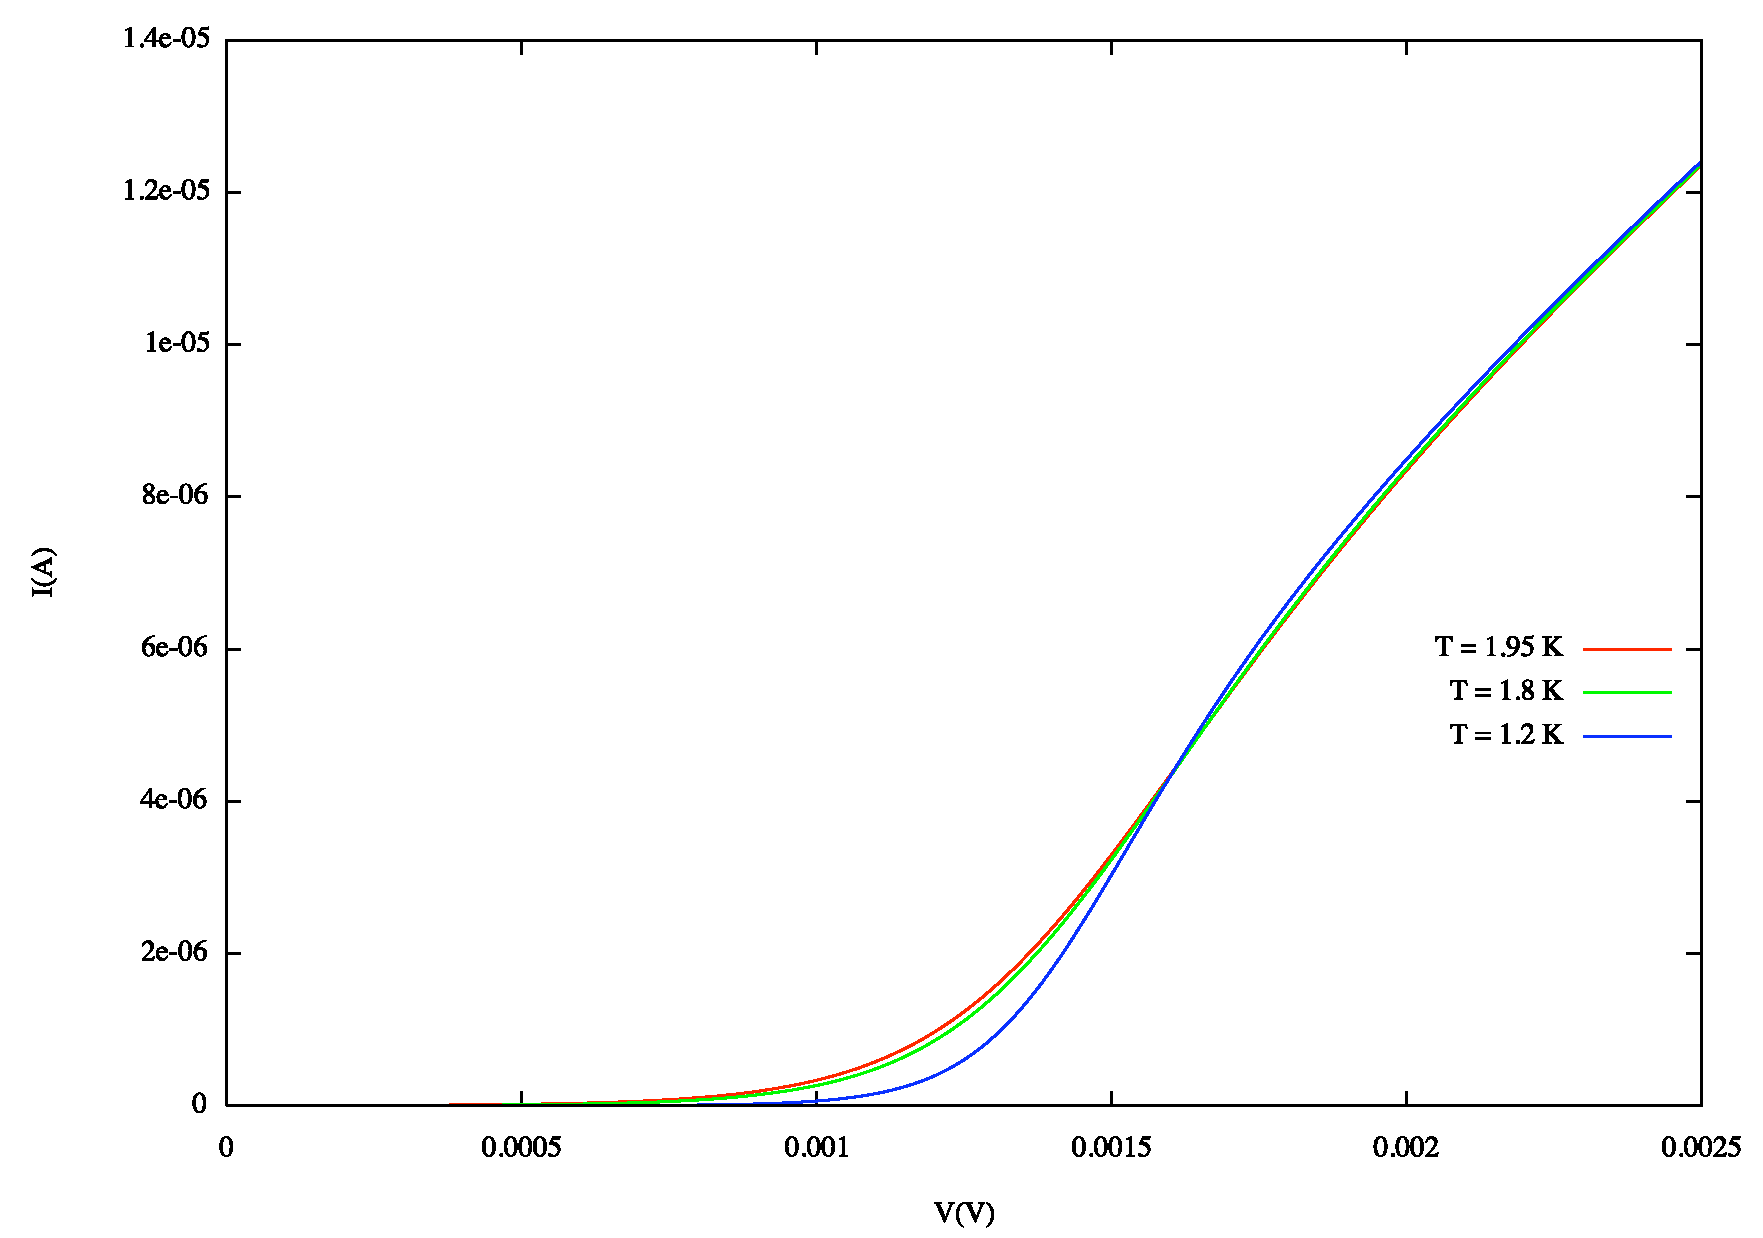
\includegraphics[width=0.45\textwidth]{iv_theoretical_4-5-10}
\caption{\small BCS theoretical current curves for different temperatures. 
\label{iv_theoretical_4-5-10}}
\end{figure}


Finally, introducing $x=E-\Delta$ and noting that Fermi functions are even, we get the expression that is used for numerical analysis:
\begin{eqnarray}\label{ins_numerical}
I^{NS} &=& \frac{C^{NN}}{e} \int_{0}^{\infty} dx\ \frac{x+\Delta}{\sqrt{x(x+2 \Delta)}} \times
		\nonumber \\
		&\times& [f(x+ \Delta-eV)-f(x+ \Delta +eV)].
		\nonumber \\
\end{eqnarray}

\begin{figure}[h!]
\centering
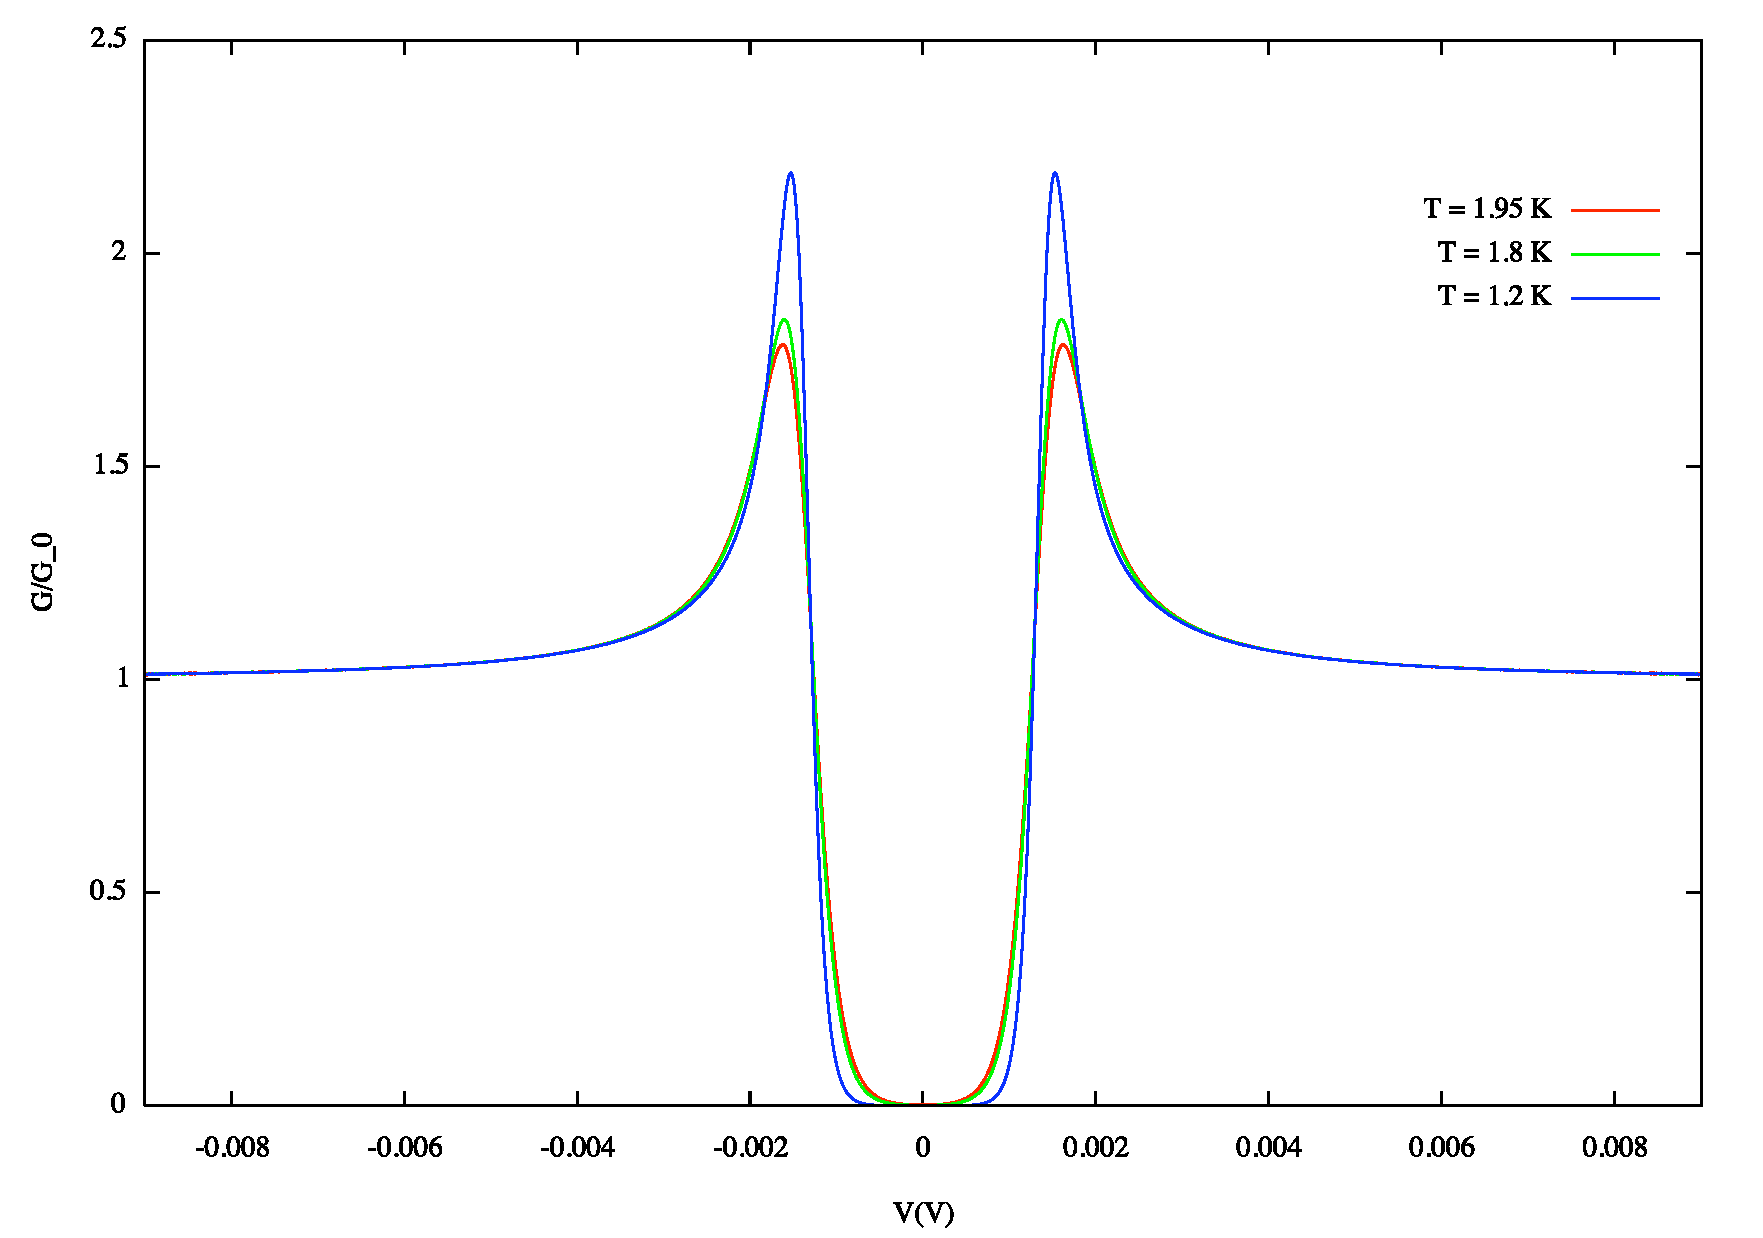
\includegraphics[width=0.45\textwidth]{gv_theoretical_4-5-10}
\caption{\small BCS theoretical conductance curves for different temperatures.
\label{gv_theoretical_4-5-10}}
\end{figure}

From \eqref{ins}, the conductance will be the following
\begin{eqnarray}\label{cns}
C^{NS} &=& \frac{1}{R^{NS}} = \frac{dI^{NS}}{dV} =
		\nonumber \\
		&=& \frac{C^{NN}}{e} \int_{-\infty}^{\infty} dE\ \frac{|E|}{\sqrt{E^2-\Delta^2}} 
		\frac{\partial f(E-eV)}{\partial V}
		\nonumber \\
\end{eqnarray}

%-----------------------------------------------------------------
\subsection{Superconductor-Superconductor junction} 
By analogy with the previous section, we write directly the expression of the current for this situation:
\begin{eqnarray}\label{iss}
I^{SS} = \frac{C^{NN}}{e} \int_{-\infty}^{\infty} dE\ 
		\frac{E^2\ [f(E-eV)-f(E)]}{\sqrt{(E^2-\Delta_1 ^2)}\sqrt{(E^2-\Delta_2 ^2)}}.
		\nonumber \\
\end{eqnarray}
